\documentclass[border=5mm,tikz]{standalone}
\usepackage{tikz-cd}
\usepackage{amsmath}

\begin{document}
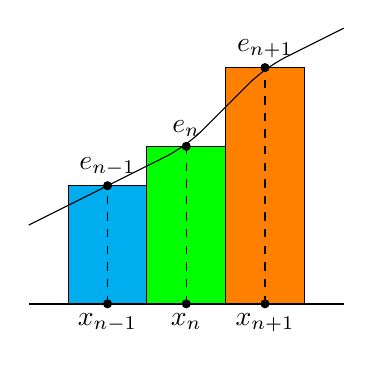
\begin{tikzpicture}

\draw[thick] (-0.5, 0) -- (3.5, 0);

\filldraw[fill=cyan] (0, 0) rectangle (1, 1.5);
\draw[dashed] (0.5, 0) -- (0.5, 1.5);
\draw[fill] (0.5, 0) circle [radius=0.05];
\node [below] at (0.5, 0) {$x_{n-1}$};
\draw[fill] (0.5, 1.5) circle [radius=0.05];
\node [above] at (0.5, 1.5) {$e_{n-1}$};


\filldraw[fill=green] (1, 0) rectangle (2, 2);
\draw[fill] (1.5, 0) circle [radius=0.05];
\node [below] at (1.5, 0) {$x_n$};
\draw[fill] (1.5, 2) circle [radius=0.05];
\node [above] at (1.5, 2) {$e_n$};
\draw[dashed] (1.5, 0) -- (1.5, 2);

\filldraw[fill=orange] (2, 0) rectangle (3, 3);
\draw[fill] (2.5, 0) circle [radius=0.05];
\node [below] at (2.5, 0) {$x_{n+1}$};
\draw[fill] (2.5, 3) circle [radius=0.05];
\node [above] at (2.5, 3) {$e_{n+1}$};
\draw[dashed] (2.5, 0) -- (2.5, 3);

\draw[rounded corners=8pt] (-0.5, 1) -- (0.5, 1.5) -- (1.5, 2) -- (2.5, 3) -- (3.5, 3.5);

\end{tikzpicture}
\end{document}